\documentclass[12pt,twoside]{article}
\usepackage{jmlda}
\newtheorem{defn}{Definition}[section]
%\NOREVIEWERNOTES
\title
[Фрактальный анализ и синтез оптических изображений морского волнения] % Краткое название; не нужно, если полное название влезает в~колонтитул
{Фрактальный анализ и синтез оптических изображений морского волнения}
\author
[Автор~И.\,О.] % список авторов для колонтитула; не нужен, если основной список влезает в колонтитул
{Каныгин~Ю.\,Ю., Лукошин~В.\,О., Фамилия~И.\,О.} % основной список авторов, выводимый в оглавление
[Каныгин~Ю.\,Ю., Лукошин~В.\,О.$^2$, Фамилия~И.\,О.$^2$] % список авторов, выводимый в заголовок; не нужен, если он не отличается от основного
\thanks
{Работа выполнена при финансовой поддержке РФФИ, проект \No\,00-00-00000.
	Научный руководитель:  Стрижов~В.\,В.
	Задачу поставил:  Матвеев~И.\,О.
	Консультант:  Консультант~И.\,О.}
\email
{author@site.ru}
\organization
{$^1$Московский физико-технический институт (Государственный Университет); $^2$Организация}
\abstract
{Работа посвящена исследованию проблемы определения спектра волн возвышений морской поверхности и его связи с фрактальной размерностью. Предложен подход определения степени спектра с помощью сверточной нейронной сети. С помощью “” подхода по определению фрактальной размерности и нейронной сети устанавливается зависимость между показателем спектра волн возвышений и фрактальной размерностью изолиний яркости.
	
	\bigskip
	\textbf{Ключевые слова}: \emph {дистанционное зондирование, аэрокосмические изображения, спектры волнения, поверхностное волнение, обработка изображений, приповерхностный слой океана, оценка фрактальной размерности
}.}
\titleEng
{Название на заморском}
\authorEng
{Author~F.\,S.$^1$, CoAuthor~F.\,S.$^2$, Name~F.\,S.$^2$}
\organizationEng
{$^1$Moscow Institute of Physics and Technology (State University); $^2$Organization}
\abstractEng
{This document is ....
	
	\bigskip
	\textbf{Keywords}: \emph{keyword, keyword, more keywords}.}
\begin{document}
	\maketitle
	%\linenumbers
	\section{Введение}
Изучение поведения поверхности океана носит важный прикладной характер. Для большинства задач контроля состояния морской поверхности требуется восстановление спектров высот и уклонов волнения по данным дистанционного зондирования, в частности по его оптическим изображениям. Такие спектры позволяют получать важную информацию о различных процессах и явлениях, происходящих на поверхности и в приповерхностном слое морей и океанов, об энергетических особенностях морских волн, о характеристиках приводного слоя атмосферы и ветровом режиме, а также выявлять зоны негативных естественных антропогенных воздействий на водную среду, свидетельствовать о чрезвычайных ситуациях в океане и др. Изучение спектра морской поверхности сложная и актуальная задача. В работе \cite{author09anyscience} было установлено, что спектр уклонов высот морской поверхности является степенным. Известно, что если спектр является степенным, то данная структура является фрактальной. Знание показателя степени спектра дает ответы на вопрос о структуре волнения. В \cite{author09anyscience} было показано, что фрактальная размерность изолинии яркости изображения морской поверхности линейно зависит от показателя спектра в исследуемом диапазоне, однако весовые функции зависят от площади изолинии. Так же в \cite{author09anyscience} был предложен алгоритм восстановления изображения морского волнения по показателю спектра. На практике, показатель спектра $p$ --- неизвестен, но есть изображение морской поверхности. Поэтому хотелось бы восстанавливать $p$ по изображению. \\
В данной работе, с помощью методов машинного обучения предлагается решение данной проблемы. С помощью алгоритма из \cite{author09anyscience} была сгенерирована выборка изображений с различными $p$  и при различных атмосферных условиях. Чтобы избавится от условий съемки, все изображения были подвергнуты линейному преобразованию (конкретнее) над полем контрастности. 
\begin{figure}[H]
    \centering
    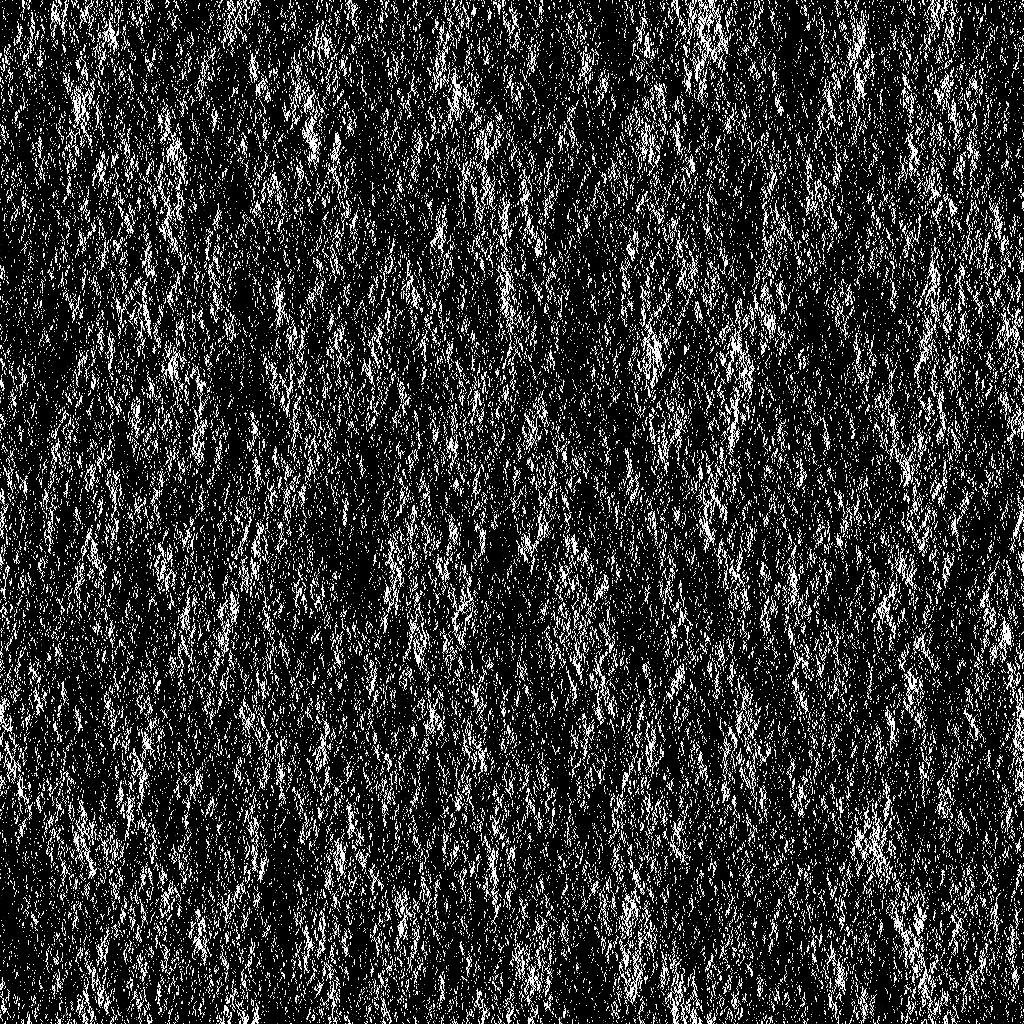
\includegraphics[width=0.6\textwidth]{p_33_W_16.eps}
    \caption{Пример изображения после преобразования над контрастностью}
\end{figure}

\section{Определение фрактальной размерности}	
Опорой при исследовании фрактальной размерности изображения была работа \cite{so2017enhancement}. Для вычисления фрактальной размерности структур нашего изображения было использовано следующее определение:

\defn[Определение фрактальной размерности]{
$$
D_2 = \dfrac{\partial\log\sum\limits_i C^2_{r,i}}{\partial\log r}, \quad  r\in \left[r_1, r_2\right]
$$
}

Получается следующий алгоритм для вычисления:
\begin{enumerate}
    \item На вход подается изображение нашего <<безобразия>>
    \item Для набора точек в $n$-мерном пространстве определяется его конечное покрытие
    \item Последнее разбивается сеткой разной мелкости. 
    \item Для каждой мелкости разбиения $r$, производится подсчёт непустых ячеек $N$ либо квадрат числа точек, оказавшихся в ячейке, $C$.
    \item Строится график $N$ либо $C$ vs. $r$ в log-log масштабе. 
    \item Наклон кривой на <<линейном>> участке является фрактальной размерностью,  которая подается на выход.
\end{enumerate}
Данная программа была апробирована на общеизвестных фракталах
\begin{figure}[H]
    \centering
    \includegraphics{test}
    \caption{Тест вычисления фракталной размерности}
\end{figure}
В частности для фрактала Серпинского:
\begin{figure}[H]
    \centering
    \includegraphics[width=\textwidth]{table.eps}
    \caption{Характеристики алгоритма вычисления фрактальной размерности для треугольника Серпинского}
\end{figure}

\begin{figure}[H]
    \centering
    \includegraphics{serpinskii}
    \caption{График $N$ vs. $r$ в log-log масштабе}
\end{figure}
\section{Постановка задачи машинного обучения}
Для практического применения, очень удачным оказывается тот факт, что в исследуемом диапазоне зависимость фрактальной размерности и показателя спектра изолиний оказывается линейной. 
$$
D\left( p\right) = \beta_o \left(n\right) + \beta_1 \left(n\right)\left(p - p_0\right)
$$
Данная задача является задачей линейной регрессии. Для ее решения, первое, что может прийти в голову --- это решение с помощью метода наименьших квадратов. На языке математики, задача представляется следующим образом:
$$
\vec{p} = f\left(\vec{\omega}, \vec{D}\right) + \vec{\nu} = \sum\limits_{i = 1}^N \omega_i D_i + \vec{\nu}
$$
Минимизация квадрата разности между фактическими занчениями переменной $D$ и восстановленной $f\left(\vec{\omega}, \vec{D}\right)$  является оптимизационной задачей, из которой находятся веса $\vec{\omega}$.
$$
S = \sum\limits_{i = 1}^N \left(f\left(\vec{\omega}, \vec{D}\right) - \vec{p}\right)^2 = \vert \vec{A}\cdot\vec{D} - \vec{p}\vert^2 \rightarrow \min
$$
$$
\vec{\omega} = \argmin\limits_{\vec{\omega \in \mathbb{R}^3}} S
$$
Хотя, вообще говороя данная задача может быть решена аналитически:
$$
\vec{\omega} = \left(\vec{A}^T \vec{A}\right)^{-1} \left(\vec{A}^T \cdot \vec{p}\right)
$$
\begin{figure}[H]
    \centering
    \includegraphics[width=0.7\textwidth]{regr.eps}
    \caption{Зависимость показателя спектра от фрактальной размерности}
\end{figure}

\section{Заключение}
План работ на следующий семестр таков:
\begin{enumerate}
    \item Хотелось бы миновать стадию определения фрактальной размерности и иметь программу, которая на входе имеет фото морского волнения, а на выходе ответ о показателе спектра.
    \item Для этого можно попробовать построить нейронную сеть. Архитектура которой, пока что нами не разработана и не продумана.
    \item Статей по близкой тематике в области машинного обучения нами найдены не были, поэтому данная работа претендует на наличие научной новизны. 
    \item  Будет возможность сравнить ответы между двумя способами: нейронной сетью и метода фрактальной размерности. 
\end{enumerate}


	\newpage
	%\bibliographystyle{unsrt}
	%\bibliography{jmlda-bib}
	\begin{thebibliography}{1}
		
		\bibitem{author09anyscience}
		\BibAuthor{Лупян\;Е.}{
		\BibTitle{Возможности фрактального анализа оптических изображений морской поверхности}~//
		\BibJournal{10-th Int'l. Conf. on Anyscience}, 2009.  Vol.\,11, No.\,1.  Pp.\,111--122.
		\bibitem{myHandbook}
 	\BibAuthor{Бондур\;В.\,Г.}{
		Методы восстановления спектров морского волнения по спектрам аэрокосмических изображений.
		Город: Издательство, 2009. 314~с.}}
     \bibitem{so2017enhancement}{
     So G. B., So H. R., Jin G. G. Enhancement of the Box-Counting Algorithm for fractal dimension estimation //Pattern Recognition Letters. – 2017. – Т. 98. – С. 53-58.}
      \bibitem{murunin}{Мурынин А. Б. Восстановление пространственных спектров морской поверхности по оптическим изображениям в нелинейной модели поля яркости //Исследование Земли из космоса. – 1990. – №. 6. – С. 60-70.}
	\end{thebibliography}
	
	% Решение Программного Комитета:
	%\ACCEPTNOTE
	%\AMENDNOTE
	%\REJECTNOTE
\end{document}